\documentclass[10pt]{article}
\makeatletter
\usepackage[numbered,autolinebreaks,useliterate]{mcode}
\usepackage{textcomp}
\usepackage{verbatim}
\usepackage{lmodern}
\usepackage{comment}
\includecomment{Answ}
\usepackage{listings}
\usepackage{color} %red, green, blue, yellow, cyan, magenta, black, white
\definecolor{mygreen}{RGB}{28,172,0} % color values Red, Green, Blue
\definecolor{mylilas}{RGB}{170,55,241}
\renewcommand\paragraph{\@startsection{paragraph}{4}{\z@}%
            {-2.5ex\@plus -1ex \@minus -.25ex}%
            {1.25ex \@plus .25ex}%
            {\normalfont\normalsize\bfseries}}
\makeatother
\usepackage{gensymb}
\setcounter{secnumdepth}{4}
\usepackage{amsmath}
%\usepackage{mathtools}
\usepackage{graphicx}
\usepackage{slashed}
\usepackage{lineno}
\usepackage{latexsym}
\usepackage{subfigure}
\usepackage{amssymb}
\newtheorem{thm}{Theorem}[section]
\newtheorem{cor}[thm]{Corollary}
\newtheorem{lem}[thm]{Lemma}
\usepackage[numbers,sort]{natbib}
\usepackage{enumerate}
\newcommand{\bb}{\begin{equation}}
\newcommand{\ee}{\end{equation}}
\newtheorem{defin}{Definition}
\usepackage{multirow}
\usepackage{ctable}
\usepackage{bm}
\usepackage{enumerate}
\newcommand{\D}[2]{\frac{\partial #1}{\partial #2}}
\newcommand{\DD}[2]{\frac{\partial^2 #1}{\partial #2^2}}
\newcommand{\UB}[2]{\underbrace{#1}_{\textrm{\parbox{8em}{\centering #2}}}}
\newcommand{\rd}{\text{ d}}
\newcommand{\disk}{}
\usepackage{framed}
\newcommand{\see}[1]{(see Figure \ref{#1})}
\newcommand{\fig}[1]{Figure \ref{#1}}
\newcommand{\figs}[2]{figures \ref{#1} and \ref{#2}}
\newcommand{\sect}[1]{Section \ref{#1}}
\newcommand{\app}[1]{Appendix \ref{#1}}
\newcommand{\chap}[1]{Chapter \ref{#1}}
\newcommand{\eqn}[1]{equation \eqref{#1}}
\newcommand{\eqns}[2]{equations \eqref{#1} and \eqref{#2}}
\newcommand{\eqnto}[2]{equations \eqref{#1}-\eqref{#2}}
%\usepackage{authblk}
\usepackage{url}
\usepackage{hyperref}
\usepackage{soul}
\newcommand{\eg}{\emph{e.g.} }
\newcommand{\bn}{\bm{n}}
\newcommand{\bu}{\bm{u}}
\newcommand{\ie}{\emph{i.e.} }
\newcommand{\Chapter}[1]{\chapter{#1}\label{#1}}
\newcommand{\Section}[1]{\section{#1}\label{#1}}
\newcommand{\Subsection}[1]{\subsection{#1}\label{#1}}
\newcommand{\Subsubsection}[1]{\subsubsection{#1}\label{#1}}
\newcommand{\Appendix}[1]{\appendix{#1}\label{#1}}
\usepackage[margin=1.5cm,centering]{geometry}
\usepackage[geometry]{ifsym}
\makeatletter
\newcommand\restr[2]{{% we make the whole thing an ordinary symbol
  \left.\kern-\nulldelimiterspace % automatically resize the bar with \right
  #1 % the function
  \vphantom{\big|} % pretend it's a little taller at normal size
  \right|_{#2} % this is the delimiter
  }}
\def\url@leostyle{%
  \@ifundefined{selectfont}{\def\UrlFont{\sf}}{\def\UrlFont{\small\ttfamily}}}
\makeatother
\urlstyle{leo}
\usepackage{multirow}
\usepackage{blkarray}
\usepackage{soul}
\usepackage{framed}
\usepackage{color}
\usepackage{setspace}
\newcommand{\ttttp}{.24\textwidth}
\newcommand{\tttp}{.32\textwidth}
\newcommand{\ttp}{.45\textwidth}
\newcommand{\tp}{.8\textwidth}
\newcommand{\tbo}{.6\textwidth}
 \usepackage[T1]{fontenc}
\usepackage[utf8]{inputenc}
\usepackage{authblk}
 \renewcommand{\l}{\left(}
\renewcommand{\r}{\right)}
%\begin{figure}[h!!!tb]
%\centering
%\subfigure[\label{Godzilla}]{\includegraphics[height=0.35\textwidth]{./Pictures/Godzilla_final_bw.png}}
%\subfigure[\label{Jaeger}]{\includegraphics[height=0.35\textwidth]{./Pictures/Jaeger_finish_bw.png}}
%\caption{\label{Monsters} The two types of monster we are going to consider are: (a) the naturally occurring Kaijus and (b) the man-made Jaegers.}
%\end{figure}
\newcounter{Counter1}

\begin{document}

\lstset{language=Matlab,%
    %basicstyle=\color{red},
    breaklines=true,%
    morekeywords={matlab2tikz},
    keywordstyle=\color{blue},%
    morekeywords=[2]{1}, keywordstyle=[2]{\color{black}},
    identifierstyle=\color{black},%
    stringstyle=\color{mylilas},
    commentstyle=\color{mygreen},%
    showstringspaces=false,%without this there will be a symbol in the places where there is a space
    numbers=left,%
    numberstyle={\tiny \color{black}},% size of the numbers
    numbersep=9pt, % this defines how far the numbers are from the text
    emph=[1]{for,end,break},emphstyle=[1]\color{red}, %some words to emphasise
    %emph=[2]{word1,word2}, emphstyle=[2]{style},    
}


\title{Problem sheet 3}
\author{Thomas E. Woolley\\Last edited on:}
\maketitle
\section{Pushing and pulling}\label{Pushing and pulling}
In this question we will be deriving the continuum movement equation behind the discretised movement schema presented in \fig{Push_pull_taxis}. Specifically, there is a local spatially dependent rate, $r$, which pushes the particles out of their current location to a neighbouring location. Namely The rate function is evaluated at the same position as the population that it is acting on, \eg the rate of jumping from  $x_i$ (to either $x_{i-1}$ or $x_{i+1}$) is $r(x_i)u(x_i)$.

Further, there is a non-local spatially dependent rate, $s$, which pulls the particles from their current location to neighbouring location. Namely, the rate function is evaluated at the position the population is jumping to, \eg the rate of jumping from $x_i$ to $x_{i+1}$ is $s(x_{i+1})u(x_i)$.

We begin as in the lectures notes, namely, consider an infinite one-dimensional interval that is discretised into points of width $\Delta x$. Each population is centred at a point $x_i$ where $i$ is an integer label and $x_{i+1}=x_i+\Delta x$. The moving population, $u$, is labelled by both its spatial location and time during its evolution, $u(x_i,t)$.  For simplicity, $u(x_i,t)=u_i$.  Members of each population are able to transition to their neighbours at rates presented in \fig{Push_pull_taxis}. 
\begin{figure}[h!!!tb]
\centering
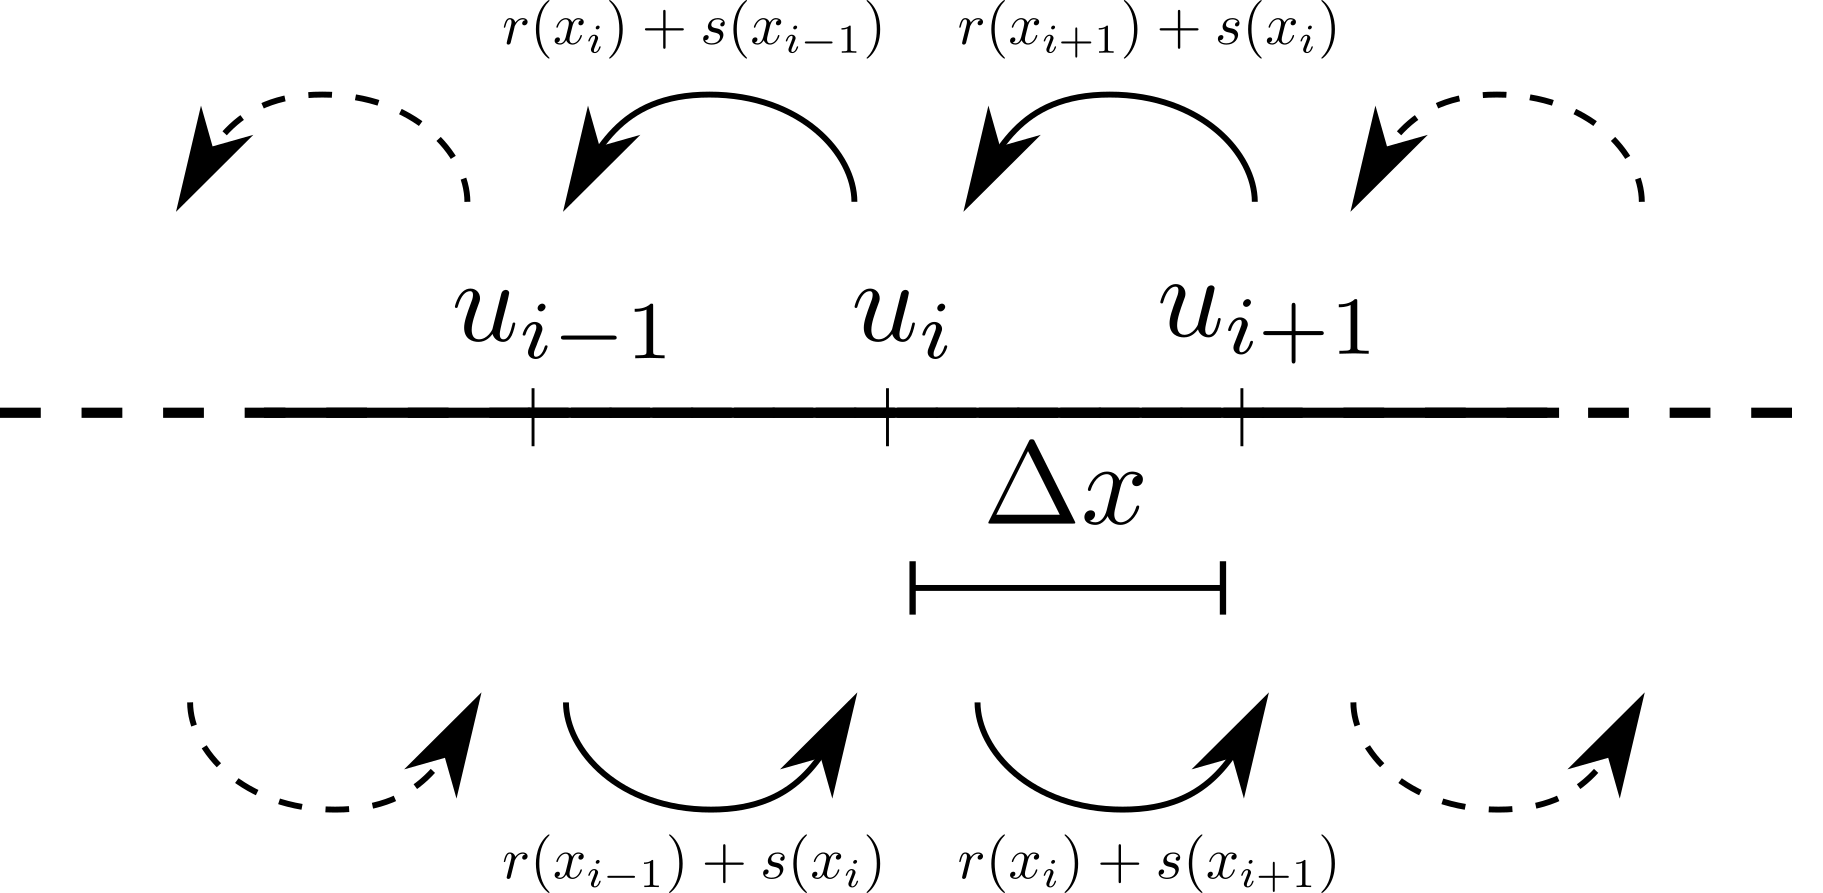
\includegraphics[width=\tp]{../../Pictures/Push_pull_taxis.png}
\caption{The push and pull movement schematic. \label{Push_pull_taxis}}
\end{figure}

\begin{enumerate}
\item Why can we ignore boundary conditions and just simply construct equations for $\dot{u}_i$?

\item Using the Law of Mass Action and \fig{Push_pull_taxis} show that the expression for $\dot{u}_i$ is
\bb
\dot{u}_i=u_{i+1}[ r(x_{i+1})+s(x_i) ]-u_i[ s(x_{i-1})+2r(x_i)+s(x_{i+1})]+u_{i-1}[ r(x_{i-1})+s(x_i) ].\label{udot}
\ee

\item Expand \eqn{udot} up to second order in $\Delta x$. Remember you will have to use Taylor series to expand $u$, $r$ and $s$. You should find the first order terms all cancel.

\item Suppose we want to take the limit of $\Delta x\rightarrow 0$ and recover a non-trivial finite limit, how should $r$ and $s$ scale with $\Delta x$? Namely, what values of $\alpha$ and $\beta$ provide a finite limit when we set $r(x)=R(x)\Delta x^\alpha$ and $s(x)=S(x)\Delta x^\beta$.

\item Substitute $r(x)=R(x)\Delta x^\alpha$ and $s(x)=S(x)\Delta x^\beta$ into the equations and show that the limiting equation is then
\bb
\D{u}{t}=\D{}{x}\l\D{u}{x}S-u\D{S}{x}\r+\DD{\l uR\r}{x}.
\ee
\item What happens in the specific case that $r=s$?
\end{enumerate}


\begin{Answ}
\subsection{Answers}
\begin{enumerate}
\item The domain is infinite, so there are no boundaries to consider. Further, by symmetry, all the points are the same. For example, if we wanted to consider $u_{i+j}=u(x_{i+j})=u(x_{i}+j\Delta x)$ we could redefine the coordinates $x_i\mapsto x_i-j\Delta x$ then $u_{i+j}$ maps to box $u_i$.

\item There are two fluxes into box $i$ and two fluxes out. Deriving each term separately, using the Law of Mass Action and \fig{Push_pull_taxis}:
\begin{itemize}
\item Flux into population $i$ from population $i-1$: $u_{i-1}[r(x_{i-1})+s(x_i)]$.
\item Flux into population $i$ from population $i+1$: $u_{i+1}[r(x_{i+1})+s(x_i)]$.
\item Flux out of population $i$ to population $i-1$: $-u_{i}[r(x_{i})+s(x_{i-1})]$.
\item Flux out of population $i$ to the population $i+1$: $-u_{i}[r(x_{i})+s(x_{i+1})]$.
\end{itemize}
Adding these terms together gives the right-hand side of \eqn{udot}.


\item Using $x_{i\pm 1}=x_i\pm\Delta x$ we can expand $u_{i\pm 1}$, using Taylor series, to get
\bb
u_{i\pm 1}=u_i\pm \Delta x\D{u_i}{x}+\frac{\Delta x^2}{2}\DD{u_i}{x}.
\ee
The functions for $r$ and $s$ can be expanded in the  same way. Substituting the expansions into \eqn{udot} gives
\begin{align}
\D{u_i}{t}=&\l u_i- \Delta x\D{u_i}{x}+\frac{\Delta x^2}{2}\DD{u_i}{x}\r\left[ r_i- \Delta x\D{r_i}{x}+\frac{\Delta x^2}{2}\DD{r_i}{x}+s_i\right]\nonumber\\
&-u_i\left[s_i- \Delta x\D{s_i}{x}+\frac{\Delta x^2}{2}\DD{s_i}{x}+2r_i+s_i+ \Delta x\D{s_i}{x}+\frac{\Delta x^2}{2}\DD{s_i}{x}\right]\nonumber\\
&+\l u_i +\Delta x\D{u_i}{x}+\frac{\Delta x^2}{2}\DD{u_i}{x}\r\left[ r_i+ \Delta x\D{r_i}{x}+\frac{\Delta x^2}{2}\DD{r_i}{x}+s_i\right],
\end{align}
which can be simplified to
\begin{align}
\D{u_i}{t}=&\l u_i(r_i+s_i)-2u_i(r_i+s_i)+u_i(r_i+s_i)\r\nonumber\\
&+\Delta x \l -(r_i+s_i)\D{u_i}{x}-u_i\D{r_i}{x}+(r_i+s_i)\D{u_i}{x}+u_i\D{r_i}{x}\r\nonumber\\
&+\Delta x^2 \l \frac{(r_i+s_i)}{2}\DD{u_i}{x}+\D{r_i}{x}\D{u_i}{x}+\frac{u_i}{2}\DD{r_i}{x}-u_i\DD{s_i}{x}+\frac{(r_i+s_i)}{2}\DD{u_i}{x}+\D{r_i}{x}\D{u_i}{x}+\frac{u_i}{2}\DD{r_i}{x}\r
\end{align}
where we have ignored terms of order higher than $\Delta x^2$. Immediately, we see that the zeroth and first order terms cancel completely, so we are left with
\bb
\D{u_i}{t}=\Delta x^2 \l r_i\DD{u_i}{x}+2\D{r_i}{x}\D{u_i}{x}+u_i\DD{r_i}{x}+s_i\DD{u_i}{x}-u_i\DD{s_i}{x}\r.\label{Expansion}
\ee


\item From considering \eqn{Expansion} we see that if $r= R/\Delta x^2$ and $s=S/\Delta x^2$ then we derive a non-trivial and non-singular equation.


\item Upon substitution of $r=R/\Delta x^2$ and $s=S/\Delta x^2$ and taking the limit $\Delta x\rightarrow 0$ we derive
\begin{align}
\D{u}{t}=& R\DD{u}{x}+2\D{R}{x}\D{u}{x}+u\DD{R}{x}+S\DD{u}{x}-u\DD{S}{x},\nonumber\\
=&\DD{\l Ru\r}{x}+S\DD{u}{x}-u\DD{S}{x},\nonumber\\
=&\DD{\l Ru\r }{x}+\D{}{x}\l S\D{u}{x}-u\D{S}{x}\r.
\end{align}

\item When $r=s$ (and $R=S$) we go back to \eqn{Expansion} to see that
\bb
\D{u_i}{t}=2\Delta x^2 \l r_i\DD{u_i}{x}+\D{r_i}{x}\D{u_i}{x}\r.
\ee
Continuing the above derivation then leads to
\bb
\D{u}{t}=2R\DD{u}{x}+2\D{R}{x}\D{u}{x}.
\ee
\end{enumerate}
\end{Answ}

\section{Travelling waves}
Foxes are territorial animals, unless they have rabies, in which case they under go random walks away from their home range. Rabies is fatal in foxes.
\begin{enumerate}
\item Justify the following equations as a model of this situation,
\begin{align}
\D{I}{t}=&D\DD{I}{x}+\alpha IS-\beta I,\\
\D{S}{t}=&-\alpha IS+rS\l 1-\frac{S}{K}\r,
\end{align}
where the populations $S$ and $I$ and the positive constants $D$, $\alpha$, $\beta$, $r$ and $K$ should be interpreted.

\item Non-dimensionalise the system to give
\begin{align}
\D{u}{\tau}=&\DD{u}{X}+uv-\mu u,\label{Rabid}\\
\D{v}{\tau}=&-uv+\gamma v\l 1-v\r\label{Healthy},
\end{align}
where $\gamma$ and $\mu$ should be defined in terms of $D$, $\alpha$, $\beta$, $r$ and $K$.

\item What are the spatially uniform steady states of system \eqref{Rabid}-\eqref{Healthy}? Explain what each steady state represents.

\item Conclude why $0<\mu<1$ must occur if a non-zero infective population is to constantly exist.

\item Convert \eqns{Rabid}{Healthy} to moving wave coordinates. Namely substitute $z=X-c\tau$, where we assume that $c$ is a positive constant. 

\item Look for a travelling wave solution that does not change shape over time.  Linearising far ahead of the wave front, where the population is fully susceptible and the infection has not yet arrived. Namely, consider expansions of the form
\begin{align}
u=&\epsilon_1\exp(\lambda z),\label{Expansionu}\\ 
v=&1+\epsilon_2\exp(\lambda z).\label{Expansionv}
\end{align}
Show that if a travelling wave exists the wave speed must satisfy $c\geq 2 \sqrt{1-\mu}$.
\end{enumerate}
\begin{Answ}
\subsection{Answers}
\begin{enumerate}
\item From inspection of the equations and the description paragraph we observe the $I$ are the rabies infected foxes, while $S$ are the susceptible foxes,
\begin{align}
\underbrace{\D{I}{t}}_{\textrm{\parbox{8em}{\centering Rate of change of infected population}}}=&\underbrace{D\DD{I}{x}}_{\textrm{\parbox{8em}{\centering Random movement of diseased population}}}+\underbrace{\alpha IS}_{\textrm{\parbox{8em}{\centering Infection rate}}}-\underbrace{\beta I}_{\textrm{\parbox{8em}{\centering Death rate}}},\\
\underbrace{\D{S}{t}}_{\textrm{\parbox{8em}{\centering Rate of change of susceptible population}}}=&\underbrace{-\alpha IS}_{\textrm{\parbox{8em}{\centering Rate of infection}}}+\underbrace{rS\l 1-\frac{S}{K}\r}_{\textrm{\parbox{8em}{\centering Natural population control through logistic growth}}},
\end{align}
Finally, $D$ is the diffusion rate, \ie the rate of random movement; $\alpha$ is the infection constant; $\beta$ is the death constant; $r$ is the growth rate; $K$ is the carrying capacity. 

\item Let $I=[I]u$, $S=[S]v$, $x=[x]X$ and $t=[t]\tau$, where the bracketed variables are the constant dimensional scales we need to define an $u, v, X$ and $\tau$ are non-dimensional variables. Substituting in and rearranging to get the left-hand side derivatives on there own:
\begin{align}
\D{u}{\tau}=&\frac{D[t]}{[x]^2}\DD{u}{X}+\alpha[S][t] uv-\beta [t]u,\label{step1u}\\
\D{v}{\tau}=&-\alpha[I][t] uv+r[t]v\l 1-\frac{[S]}{K}v\r.\label{step1v}
\end{align}
By comparing \eqns{step1u}{step1v} to \eqns{Rabid}{Healthy} we can then extract the required scales. Specifically:
\begin{itemize}
\item the logistic term tells us $[S]=K$;
\item the infection terms tell us that $\alpha[S][t]=\alpha[I][t]=1$, \ie $[S]=[I]$ and $[t]=1/(K\alpha)$;
\item the diffusion term tells us that $1=D[t]/[x]^2$, so, $[x]=\sqrt{D/(K\alpha)}$;
\item The coefficient of the death rate is $\mu=\beta[t]=\beta/(K\alpha)$ and the coefficient of the logistic term is $\gamma=r[t]=r/(K\alpha)$.
\end{itemize}
\item Steady states imply the time derivatives are zero. Spatially uniform steady states imply the spatial derivative is zero. Hence, we are looking for solutions of
\begin{align}
0=&uv-\mu u,\label{stst1}\\
0=&-uv+\gamma v\l 1-v\r.\label{stst2}
\end{align}
Solving \eqns{stst1}{stst2} simultaneously we derive that there are three steady states:
\begin{itemize}
\item $(0,0)$ is the fully extinct steady state. Namely, all of the susceptible foxes have caught rabies and eventually die.
\item $(0,1)$ is the disease eradicated case. Namely, rabies has been removed from the fox population.
\item $(\gamma(1-\mu),\mu)$ is the steady infection case.  In this case it is possible to balance the number of infections, deaths and reproductions such that all populations exist.
 \end{itemize}
 
 
 \item If we want $(\gamma(1-\mu),\mu)$ to exist then, since we are dealing with a population both populations must be non-negative, hence $\mu<1$.


 \item Defining a travelling frame of reference coordinate system $(z,\tau')$, where $z=X-c\tau$ and $\tau'=\tau$ we use the chain rule,
 \begin{align}
 \D{}{\tau}=&\D{}{\tau'}\D{\tau'}{\tau}+\D{}{z}\D{z}{\tau},\nonumber\\
 =&\D{}{\tau'}-c\D{}{z},\label{coordtau}
 \end{align}
and
 \begin{align}
 \D{}{x}=&\D{}{x}\D{\tau'}{x}+\D{}{z}\D{z}{x}\nonumber\\
 =&\D{}{z},\nonumber\\
\textrm{further implying that } \DD{}{x}=&\DD{}{z}.\label{coordx}
 \end{align}
 Dropping primes without loss of generality and substituting \eqns{coordtau}{coordx} into \eqns{Rabid}{Healthy} provides
\begin{align}
\D{u}{\tau}-c\D{u}{z}=&\DD{u}{z}+uv-\mu u,\label{Travellingu}\\
\D{v}{\tau}-c\D{v}{z}=&-uv+\gamma v\l 1-v\r\label{Travellingv}.
\end{align}


\item Looking for a stationary profile travelling wave means we can ignore the $\tau$ derivative. We now substitute expansions \eqref{Expansionu} and \eqref{Expansionv} into \eqns{Travellingu}{Travellingv} and expand to order 1 in $\epsilon_1$ and $\epsilon_2$,
\begin{align}
0=&\epsilon_1\lambda^2\exp(\lambda z)+c\epsilon_1\lambda\exp(\lambda z)+\epsilon_1\exp(\lambda z)-\mu \epsilon_1\exp(\lambda z),\label{c_eqn}\\
0=&c\epsilon_2\lambda\exp(\lambda z)-\epsilon_1\exp(\lambda z)-\gamma \epsilon_2\exp(\lambda z).
\end{align}
We could create a matrix equation out of this and set the determinant of the matrix to zero to ensure non-trivial solutions for $(\epsilon_1,\epsilon_2)$,
\bb
\left[ \begin{array}{cc}\lambda^2+c\lambda +1-\mu &0\\
-1&c\lambda-\gamma
\end {array} \right]\l \begin{array}{c}\epsilon_1\\
\epsilon_2
\end {array} \r=0,
\ee
However, it is easiest to consider \eqn{c_eqn} in this case as the $\epsilon_1 \exp(\lambda z)$ term factors out,
\bb
\lambda^2+c\lambda +1-\mu=0.\label{lambda}
\ee
For a travelling wave to be possible we need the full susceptible state to be stable with respect to $z\rightarrow \infty$, which represents  $\tau \rightarrow-\infty$. Equally, we need the steady state to be a node, not a spiral. Specifically, if the $u$ population spirals near zero it will go negative, which is unrealistic.

Thus, for this state to be a stable node we need $\lambda$ to be real and negative, so the perturbations decay. The solutions of \eqn{lambda} are
\bb
2\lambda_\pm=-c\pm\sqrt{c^2-4(1-\mu)}.
\ee
To be real we require $c^2>4(1-\mu)$ and since $c>0$ we get the inequality. To have both roots be negative we require $4(1-\mu)>0$, which makes the term inside the square root smaller than $c^2$, hence $\lambda_-<\lambda_+<0$. Since 
\bb
4(1-\mu)>0 \implies 1>\mu,
\ee
then the nontrivial steady state exists and, thus, in this case, the travelling wave may not link (0,1) to (0,0), but rather it may link (0,1) to the third steady state, $(\gamma(1-\mu),\mu)$, Hence, if the death rate $\mu$ is small enough the population may not die out, but rather live with constant possibility of infection.

\end{enumerate}
\end{Answ}




\section{Simulating diffusion}
Matlab has inbuilt codes that allow you to simulate one-dimensional partial differential equations easily. However, in this example, we will show that the discretised approximation also produces a good approximation to the diffusion equation.

From the notes we saw that the diffusion equation,
\bb
\D{u}{t}=D\DD{u}{x},
\ee
 with zero-flux boundary conditions can be discretised into the following form
\begin{align}
\D{u_1}{t}=&du_{2}-du_1,\label{u1}\\
\D{u_i}{t}=&du_{i-1}-2du_i+du_{i+1},\\
\D{u_N}{t}=&du_{N-1}-du_N\label{u2}.
\end{align}
where $d=D/\Delta x^2$ is the ratio of the diffusion constant and the discretised domain's individual box size. Equations \eqref{u1}-\eqref{u2} form a large coupled system of ODEs. Thus, we can use \texttt{ode45} to simulate the system. This is what the code below does.

Note that in this code we plot the solution in two different ways. One way (lines 32-40) is the standard space concentration graph. Namely, we fix a time and plot the solution at the time. The second way (lines 22-29) involves creating a space-time plot which shows all of the solution at once and uses the colour channel to plot the concentration as a surface.

\begin{itemize}
\item Try decreasing \texttt{dx} in line 9. This should make the solution smoother.
\item Try making an animation of the solution over time by using a \texttt{for} loop, which  increments the time value of the solution and creates a plot at each time step.
\end{itemize}

\lstset{numbers=none}
\begin{lstlisting}
%% Ensure we start from a blank slate
clear all
close all
clc

%% Initialise variables
fs=15; % Set fontsize

dx=0.1; % Set box size
T_steps=1000; % Set number of time steps over which the solution is evaluated
x=0:dx:1; % Create the spatial discretisation
N=length(x); % Defines how many ODEs there will be
t=linspace(0,1,T_steps); % Create time series
ICs=zeros(N,1); % Initialise initial condition to be a zero vector
ICs(1)=2; % Put a value of 2 in the first box as the initial condition

%% Solve the N coupled ODEs
[t,y]=ode45(@(t,y)ODE(t,y,N,dx),t,ICs);


%% Plot space-time graph
figure('units','normalized','position',[0 0 1 1/3])
subplot(1,2,1)
pcolor(x,t,y)
shading interp
xlabel('Space')
ylabel('Time')
colorbar
set(gca,'fontsize',fs)

%% Plot spatial profile over a number of time points
subplot(1,2,2)
plot(x,y(1,:))
hold on
plot(x,y(floor(T_steps/10),:))
plot(x,y(T_steps,:))
legend('$t=0$',['$t=$ ',num2str(t(floor(T_steps/10)))],['$t=$ ',num2str(t(floor(T_steps)))])
xlabel('Space')
ylabel('$u$')
set(gca,'fontsize',fs)






function dydt=ODE(t,y,N,dx)
D=0.1; % Diffusion rate

% First and last box are set with Neumann boundary conditions
dydt(1,1)=D/dx^2*(-y(1)+y(2));
dydt(N,1)=D/dx^2*(y(N-1)-y(N));

% Fill in all other vector values
for i=2:N-1
    dydt(i,1)=D/dx^2*(y(i-1)-2*y(i)+y(i+1));
end

end
\end{lstlisting}




\section*{Exam Revision}

\section{Nonlocal diffusion}
Consider a population moving on a discretised infinite domain that is able to jump to one of its three neighbouring boxes with rate $d$ \see{Nonlocal_motion}.
\begin{figure}[h!!!tb]
\centering
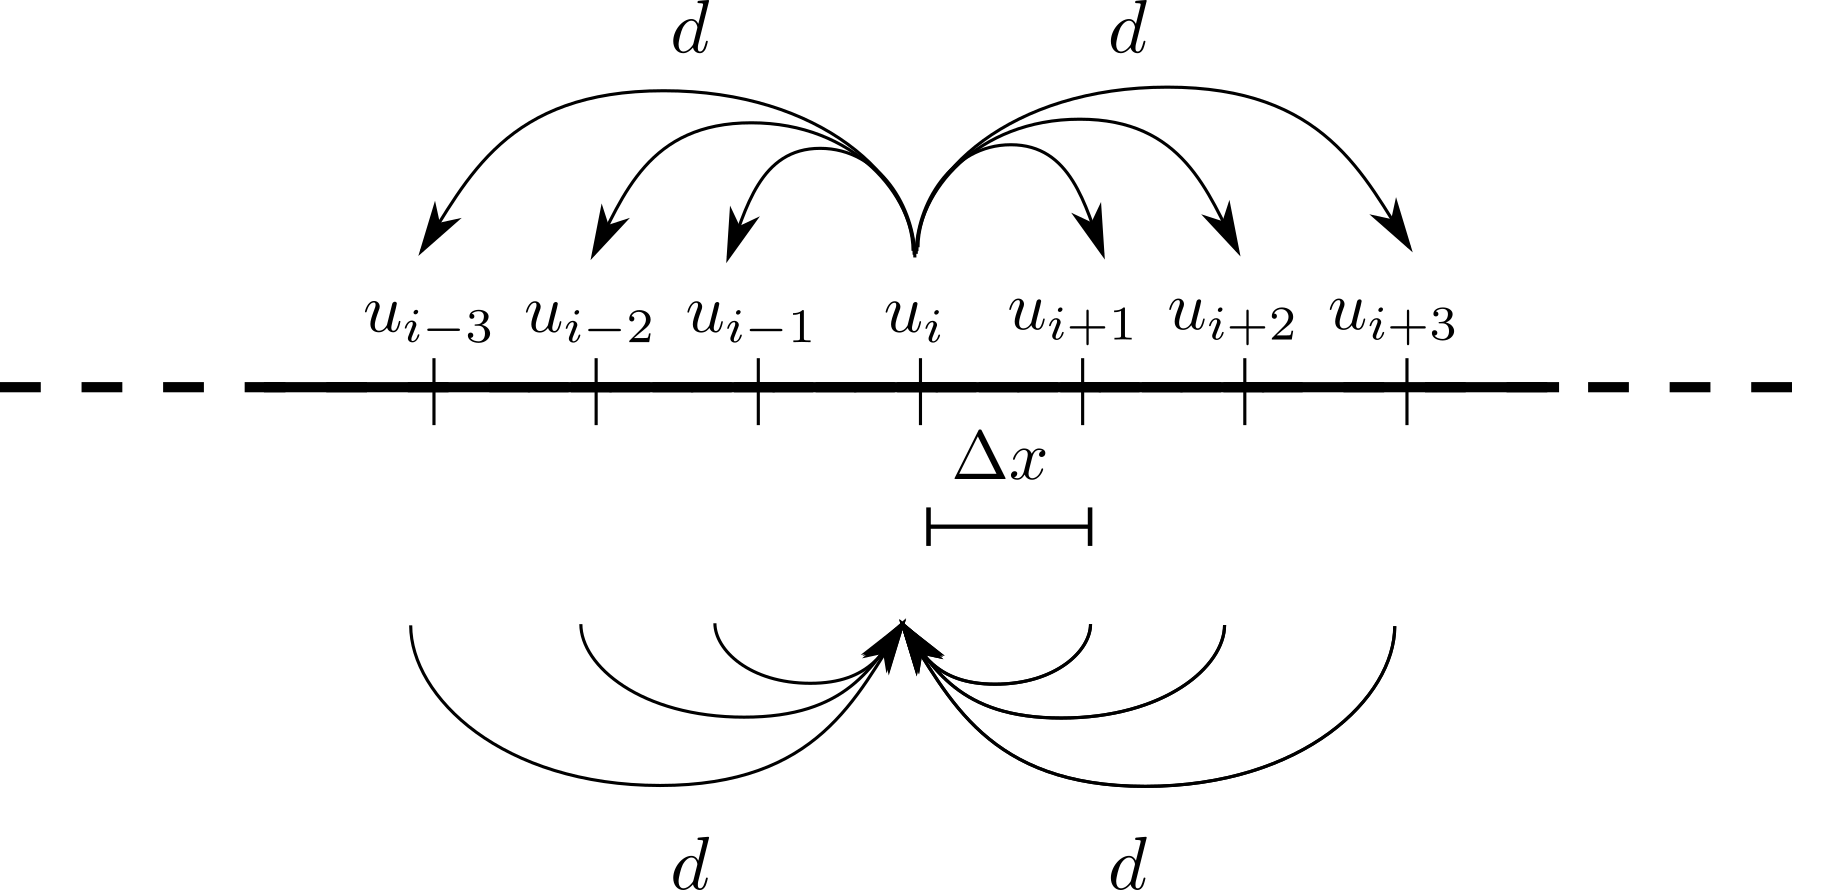
\includegraphics[width=\tp]{../../Pictures/Nonlocal_motion.png}
\caption{Nonlocal motion. Note that the population can jump to any of its neighbouring three populations. This is true for all boxes, but only movement to and from population $i$ is shown for clarity. \label{Nonlocal_motion}}
\end{figure}
\begin{enumerate}
\item Before we begin the question what PDE do you think is behind this system?

\item Write down the ODE for $u_i$.

\item Using Taylor series expand the $u_i$ ODE in terms of $\Delta x$.

\item How should $d$ scale with $\Delta x$ to produce a nonsingular and nontrivial equation?

\item Derive the PDE limit of the ODE when $\Delta x \rightarrow 0$.

\item Does the PDE you derived match your intuition?
\end{enumerate}

\begin{Answ}
\subsection{Answers}
\begin{enumerate}
\item \label{Intuition} The process is essentially three diffusions piled on top of each other, so we might guess that the final equations might be something like
\bb
\D{u}{t}=d_1\DD{u}{x}+d_2\DD{u}{x}+d_3\DD{u}{x}.
\ee
But what are $d_1$, $d_2$ and $d_3$? A simple guess would be $d_1=D$, $d_2=2D$ and $d_3=3D$, where $D$ is some scaled version of $d$, resulting in the equation
\bb
\D{u}{t}=6D\DD{u}{x}.
\ee
Note we do not know if this is right, but it can compare the final derivation with this and see what aligns with our intuition. Equally, it may suggest where we may have made a mistake if we do not derive something like the above. Again, we may not be wrong in our derivation, but it serves to highlight the unintuitive aspects.

\item For box $i$ we have the following
\bb
\dot{u}_i=d(u_{i-1}+u_{i-2}+u_{i-3}-6u_i+u_{i+1}+u_{i+2}+u_{i+3}).
\ee

\item Noting that
\bb
u_{i\pm n}=u(x_i\pm n\Delta x)
\ee
and that
\bb
f(u+a\epsilon)=f(u)+a\epsilon f'(u)+\frac{a^2\epsilon^2}{2}f''(u)+O(\epsilon^3)
\ee
we are able to derive
\begin{align}
\D{u_i}{t}=&d\l u_{i}-\Delta x\D{u_i}{x}+\frac{1}{2}\Delta x^2\DD{u_i}{x}\right.\nonumber\\
&+u_{i}-2\Delta x\D{u_i}{x}+\frac{4}{2}\Delta x^2\DD{u_i}{x}\nonumber\\
&+u_{i}-3\Delta x\D{u_i}{x}+\frac{9}{2}\Delta x^2\DD{u_i}{x}\nonumber\\
&-6u_i\nonumber\\
&+u_{i}+2\Delta x\D{u_i}{x}+\frac{4}{2}\Delta x^2\DD{u_i}{x}\nonumber\\
&\left.+u_{i}+3\Delta x\D{u_i}{x}+\frac{9}{2}\Delta x^2\DD{u_i}{x}\r,\nonumber
\end{align}
which simplifies to
\bb
\D{u_i}{t}=14d\Delta x^2\DD{u_i}{x}.\label{Discrete_diff}
\ee

\item If we let $d\propto 1/\Delta x^2$ then \eqn{Discrete_diff} has a nonsingular and nontrivial continuum limit. Let $D$ be the coefficient of proportionality.

\item Letting $\Delta x$ tend to zero we recover
\bb
\D{u}{t}=14D\DD{u}{x}.
\ee

\item Yes, or no depending on your intuition. However, in answer \ref{Intuition} we got the right form of the solution, but the wrong coefficient. Namely, we predicted that $d_1=D$, $d_2=2D$ and $d_3=3D$, whereas when we use the Taylor series we find that the jumping distances become squared because we have to expand to second order since the first order evaluates to zero. Thus, $d_1=D$, $d_2=2^2D$ and $d_3=3^2D$ resulting in the correct diffusion coefficient of $14D=D+4D+9D$.


\end{enumerate}
\end{Answ}



\section{Nonlinear travelling wave}
Consider a population of cells on an infinite one-dimensional domain that undergo logistic growth, but whose diffusion depends linearly on their density,
\bb
\D{u}{t}=\D{}{x}\l u\D{u}{x}\r+u(1-u).
\ee
The boundary conditions are $u(-\infty,t)=1$ and $u(\infty,t)=0$ and the initial condition is such that the wave has not entered into the positive $x$-axis $u(x,0)=0$ for all $x>0$, \ie the population is invading an empty space.
\begin{enumerate}
\item Convert the equation into travelling wave coordinates, $z=x-ct$, where $c>0$.
\item Suppose there is a travelling wave solution with stationary profile, which is constrained to have the form $u_z=c(u-1)$. Show there there is an exact solution for one value of the wave speed, c, which you should state.
\item By solving $u_z=c(u-1)$ subject to the boundary conditions $u(-\infty,t)=1$ and $u(A,t)=0$ and initial conditions $u(x,0)=0$ show that such a solution must be piecewise continuous \ie
\bb
u=\left\{\begin{array}{c}
u(z) \textrm{ for } z<A\\
0 \textrm{ for } z\geq A\\
\end{array}\right.
\ee
where $u(z)$ and $A$ should be found.
\item Sketch what the travelling wave solution will look like.\label{Sketch_question}
\end{enumerate}

\begin{Answ}
\subsection{Answers}
\begin{enumerate}
\item Using the standard conversion process
\bb
\D{u}{t}-c\D{u}{z}=\D{}{z}\l u\D{u}{z}\r+u(1-u).\label{Density_dependent_fisher}
\ee

\item Since we are looking for a travelling wave with a stationary profile the $t$ derivative is dropped. Equally, since $u_z=c(u-1)$ then
\bb
u_{zz}=cu_z=c^2(u-1).
\ee
Substituting these constraints into \eqn{Density_dependent_fisher} we get
\begin{align}
0=&c^2(u-1)+c^2u(u-1)+c^2(u-1)^2+u(1-u), \quad \textrm{(since $u\not\equiv 1$ we divide through be the term $u-1$)} \nonumber\\
\implies 0=&c^2+c^2u+c^2(u-1)-u,\nonumber\\
\implies 0=&2c^2u-u, \quad \textrm{(since $u\not\equiv 0$ we divide through be the term $u$)}\nonumber \\
\implies &c=\frac{1}{\sqrt{2}}.
\end{align}

\item The general  solution of $u_z=c(u-1)$ is
\bb
u(z)=B\exp(cz)+1.
\ee
The constant $B$ is fixed by knowing an initial condition, say at $z=0$. Although, $z=0$ corresponds to many points the answers should be the same at all points because the wave profile is stationary. We will simply take $x=0$ and $t=0$. Using the initial condition from the question $u(x,0)=0$, this means that $B=-1$.

We now consider the boundary conditions of the initial system. As $z\rightarrow-\infty$ we have that $u\rightarrow 1$. This is automatically satisfied for all $B$ as $\exp(cz)\rightarrow 0$ for all $c>0$. As $z\rightarrow \infty$ we have that $u(z)\rightarrow 0$. However, $u(z)\rightarrow-\infty$, which is not possible. Thus, we create a piecewise solution, namely,
\bb
u(z)=\left\{\begin{array}{l}1-\exp(cz)  \textrm{ for } z<A,\\0 \textrm{ for } z\geq A.\end{array}\right.
\ee
To ensure continuity $A$ is the point at which
\begin{align}
0=&1-\exp(cA),\\
\implies A=&0.
\end{align}
Thus, a travelling wave solution to the original to the original equation is
\bb
u(x,t)=\left\{\begin{array}{l}1-\exp(c(x-ct))  \textrm{ for } x<ct,\\0 \textrm{ for } x\geq ct,\end{array}\right.
\ee
where $c=1/\sqrt{2}$.
\item See \fig{Exponential_travelling_wave.png}. We see that the profile has a negative exponential shape until it hits $u=0$, where thereafter it is identically zero.
\begin{figure}[h!!!tb]
\centering 
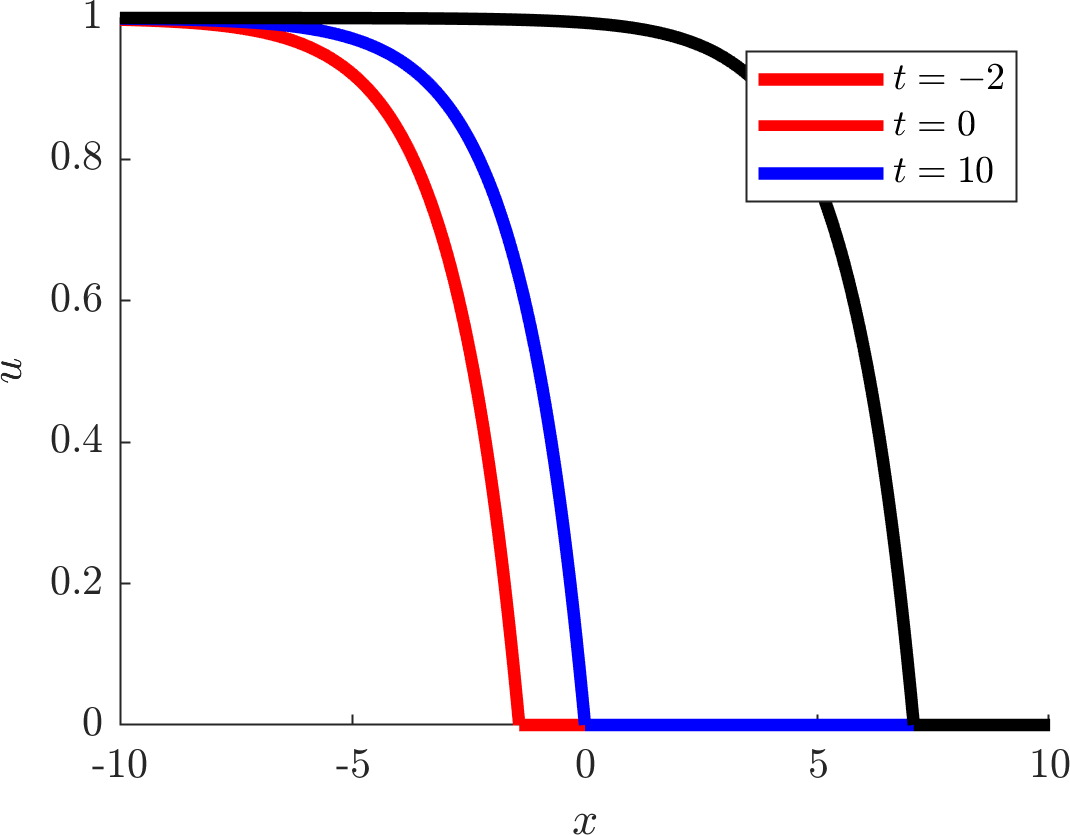
\includegraphics[width=\ttp]{../../Pictures/Exponential_travelling_wave.png}
\caption{Solution to question \ref{Sketch_question}. \label{Exponential_travelling_wave.png}}
\end{figure}
\end{enumerate}
\end{Answ}

\end{document}